\documentclass[12pt]{article}
\usepackage{graphicx}
    \usepackage[
        twoside,
        top=1in,
        bottom=0.75in,
        inner=0.5in,
        outer=0.5in
    ]{geometry}
\begin{document}
\section{Robot Control Exam, Task 2 – DH convention, FK, IK}

Given the visual description of the kinematic chain, consisting of:
\begin{enumerate}
    \item prismatic joint attached to base with actuation $d_1$ from 0 to 1 right 
    \item link: $a_1$ right, $a_2$ up, $a_3$ right
    \item revolute joint with actuation $\theta$ from 0 to $2\pi$
    \item link: $a_4$ up, $a_5$ right
    \item prismatic joint with actuation $d_2$ from 0 to 1 downwards
    \item link: $a_6$ down, ending with the end-effector
\end{enumerate}
\begin{center}
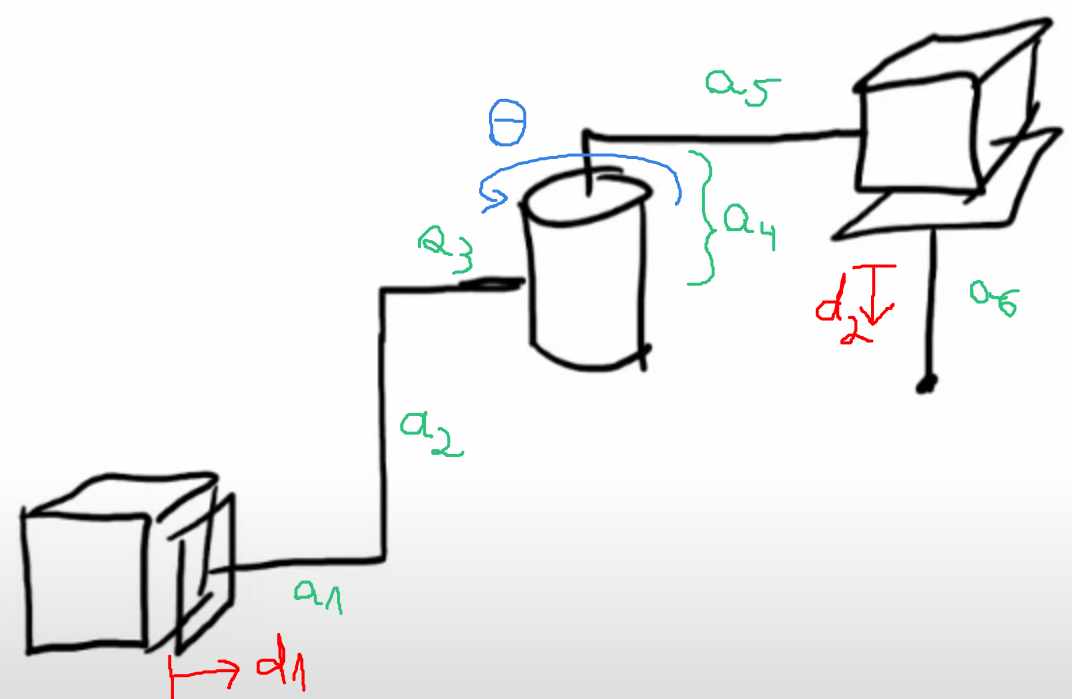
\includegraphics[scale=0.3]{theory-2.png}
\end{center}
Please do:
\begin{enumerate}
    \item Find the forward kinematics $FK(d_1, \theta, d_2)$ of the robot 
    \item Find the workspace of the robot with fixed $d_1 = 0$
    \item Find the inverse kinematics of the robot with fixed $d_1 = 0$, ie. $IK(x, y, z) = (\theta, d_2)$, such that $FK(0, \theta, d_2) = (x, y, z)$
    \item Assign frames to the joints of the kinematic chain using the DH-convention
    \item Create the DH-table for the kinematic chain including the actuation of joints
\end{enumerate}
Each subtask is worth $20\%$ of points for the task.  

\end{document}

